% !TeX program = xelatex
% UTF-8. Compile from this directory: xelatex "Low Back Pain.tex"
% Define \LBPInNotebook before \input to use within an existing XePersian document.
% Source: Google Drive Notebook/LBP; original files ordered by handwritten page number.
% images/pic01.jpg = 20261011_121936923.jpg; Drive ID: 1cikEIAM4jwlFD6uQlut5Qxpl1DhjSpCt
% images/pic02.jpg = 20261011_121953940.jpg; Drive ID: 1-cX9XhTTXepyg6isGKFKz-Bfjk2ElqMt
% images/pic03.jpg = 20261011_121958501.jpg; Drive ID: 1l63COEzF7bDS35TCWRSGLEHnBR3dZTyL
% images/pic04.jpg = 20261011_122010577.jpg; Drive ID: 1BeiSU3XXC5v311YvSr004VH4A3YmMjxF
% images/pic05.jpg = 20261011_122015587.jpg; Drive ID: 1pr4ju42_0lTmEGHeLk4X-r8L6oJgw4Jy
\ifdefined\LBPInNotebook
  \let\LBPfinish\relax
\else
  \def\LBPfinish{\end{document}}
  \documentclass[12pt,a4paper]{article}
  \usepackage[margin=22mm]{geometry}
  \usepackage{amsmath,amssymb}
  \usepackage{graphicx}
  \usepackage{array,longtable}
  \usepackage{xepersian}
  \IfFontExistsTF{Amiri}{\settextfont{Amiri}}{\settextfont{DejaVu Sans}}
  \setlatintextfont{DejaVu Serif}
  \setlength{\parindent}{0pt}
  \setlength{\parskip}{5pt}
  \setlength{\emergencystretch}{3em}
  \begin{document}
\fi
\providecommand{\LBPpage}[1]{\clearpage\section*{تصویر #1}}
\providecommand{\LBPunclear}[1]{\textbf{[خوانش نامطمئن: #1]}}
\providecommand{\LBPm}[1]{\lr{\(#1\)}}

\begin{center}\Large\bfseries\lr{Low Back Pain}\end{center}
% All medical statements below are transcriptions of the source, not corrected recommendations.
% Branches and braces in the handwritten diagrams are represented by lists and tables.

\LBPpage{۱}
\textbf{سربرگ:} \lr{No. Back pain}؛ \lr{Date} خالی؛ نشان \lr{PAPCO}؛ شمارهٔ دست‌نویس: ۱.
\subsection*{ارزیابی \lr{Low Back Pain} در بزرگسالان}
۸۴\% بزرگسالان در طول زندگی \lr{LBP} را تجربه می‌کنند.

\textbf{تقسیم‌بندی زمانی:}
\begin{itemize}
  \item \lr{Acute}: تا ۴ هفته.
  \item \lr{Subacute}: ۴ تا ۱۲ هفته.
  \item \lr{Chronic}: تا بیش از ۱۲ هفته.
\end{itemize}
ندرتاً \lr{Back Pain} بیانگر یک بیماری جدی می‌باشد.

\subsection*{ترمینولوژی}
\begin{itemize}
  \item \lr{Spondylosis}: آرتریت \lr{Spine}، یک یافتهٔ رادیولوژیک است؛ کاهش فضای دیسک‌ها و تغییرات سطح \lr{facet joints}.
  \item \lr{Anterolisthesis}: جابه‌جایی قدامی مهره نسبت به مهرهٔ پایینی.
  \item \lr{Spondylolisthesis}: انترلیستزیس ثانویه به اسپوندیلولایزیس.
  \item \lr{Retrolisthesis}: جابه‌جایی خلفی بادی مهره نسبت به مهرهٔ پایینی.
\end{itemize}
\textbf{گریدهای لیستزیس:}
\begin{center}
\begin{tabular}{|c|c|c|}
\hline
گرید & میزان لغزش & درمان (براکت منبع) \\
\hline
\lr{I} & \lr{1--25\% Slip} & \lr{Non-surgical} \\
\lr{II} & \lr{26--50\% Slip} & \lr{Non-surgical} \\
\lr{III} & \lr{51--75\% Slip} & \lr{Surgical} \\
\lr{IV} & \lr{76--100\% Slip} & \lr{Surgical} \\
\hline
\end{tabular}
\end{center}
\begin{itemize}
  \item \lr{Spondylolysis}: شکستگی در اینترآرتیکولاریس.
  \item \lr{Spinal Stenosis}: باریک شدن کانال نخاعی.
  انواع: \lr{Local, Segmental, General}.
  شایع‌ترین علت: تغییرات در سطح \lr{facet j} به علت هایپرتروفی.
  \item \lr{Radiculopathy}: \lr{Impairment of the nerve root}.
  علائم: \lr{radiating pain, numbness, tingling}، ضعف عضلانی.
  \item \lr{Cauda Equina Synd}: \lr{Loss of bowel and Bladder Control}، ضعف عضلات \lr{lower}.
  \item \lr{Kyphosis}: انحنای خارجی ستون مهرهٔ توراسیک.
  \item \lr{Lordosis}: انحنای داخلی ستون مهرهٔ لومبار.
  \item \lr{Scoliosis}: انحنای جانبی ستون مهره؛ همواره غیرطبیعی است.
\end{itemize}

\LBPpage{۲}
\textbf{سربرگ:} \lr{No.} و \lr{Date} خالی؛ \lr{PAPCO}؛ شماره: ۲.
\subsection*{ریسک فاکتورهای مرتبط با \lr{Back pain}}
سیگار، چاقی، سن، جنسیت زن، شغل استرس‌زا، شغل \lr{sedentary}، عدم رضایت شغلی.
شاخهٔ مرتبط با شغل استرس‌زا: استرس فیزیکی و وضعیت سایکولوژیک.

اختلالات سایکولوژیک: اضطراب، افسردگی، اختلالات \lr{Somatization}.

\subsection*{اتیولوژی‌های \lr{Low Back Pain}}
\textbf{\lr{Urgent and acute}:}
\begin{itemize}
  \item فشار بر طناب نخاعی به هر علتی / \lr{CES}: \lr{MRI w/o}.
  \item کنسر متاستاتیک: \lr{MRI with and w/o}؛ \lr{ESR, CRP}.
  \item آبسهٔ اپی‌دورال / استئومیلیت مهره: \lr{MRI with and w/o}؛ \lr{ESR/CRP} و کشت.
  \item شکستگی فشردهٔ مهره: رادیوگرافی لومبوساکرال.
  \item رادیکولوپاتی: اگر بیش از ۱ عصب درگیر باشد، \lr{MRI}.
\end{itemize}
\textbf{\lr{Subacute and chronic}:}
\begin{itemize}
  \item \lr{Spinal Stenosis}.
  \item اسپوندیلوآرتریت محوری (\LBPunclear{آنکیلوزال}).
  \item استئوآرتریت.
  \item اسکولیوز / کیفوز.
\end{itemize}
مهم‌ترین اتیولوژی \lr{LBP}، علل غیراختصاصی (\lr{nonspecific}) است؛ ۸۵\% موارد را تشکیل می‌دهد.

\subsection*{ضایعات منفرد ریشه‌های عصبی}
\begin{latin}
\small
\setlength{\tabcolsep}{4pt}
\renewcommand{\arraystretch}{1.25}
\begin{longtable}{|p{0.07\textwidth}|p{0.23\textwidth}|p{0.22\textwidth}|p{0.24\textwidth}|p{0.13\textwidth}|}
\hline
Root & Pain & Sensory loss & Weakness & Stretch reflex loss \\
\hline
\endhead
L\textsubscript{1} & Inguinal region & Inguinal region & rarely hip reflex & Non \\
\hline
L\textsubscript{2}--L\textsubscript{3}--L\textsubscript{4} & Back radiating into anterior Thigh & & Hip flexion, hip adduction, knee extension & Patellar tendon \\
\hline
L\textsubscript{5} & Back radiating into buttock, lateral thigh, lateral calf, great toe & lateral calf, first web space & Hip abduction, knee flexion, foot dorsiflexion & Semi\-tendinosus \\
\hline
S\textsubscript{1} & Lateral or posterior thigh & posterior thigh, lateral or plantar aspect of foot & Knee flexion, plantar flexion & Achilles tendon \\
\hline
S\textsubscript{2}--S\textsubscript{3}--S\textsubscript{4} & Sacral pain, posterior aspects of the leg & Medial buttock, perianal region & Incontinence & Anal wink \\
\hline
\end{longtable}
\end{latin}
\textbf{یادداشت خوانش:} در سطر \lr{L\textsubscript{1}} عبارت دست‌نویس \lr{rarely hip reflex} و \lr{Non} آمده است؛ عبارت بدون اصلاح حفظ شده است. سطر \lr{L\textsubscript{2}--L\textsubscript{4}} چهار گروه متن پس از ریشه دارد و ستون حس در منبع جداگانه نوشته نشده است.

\LBPpage{۳}
\textbf{سربرگ:} \lr{No.} و \lr{Date} خالی؛ \lr{PAPCO}؛ شماره: ۳.
\subsection*{رویکرد به بیمار \lr{LBP} حاد}
شاخه‌ها به ترتیب فلش‌های منبع:
\begin{enumerate}
  \item شواهد \lr{CES}: احتباس ادراری، بی‌اختیاری یا \LBPunclear{سدل آنستزی} یا ضعف پای پیش‌رونده.
  اگر بله، \lr{MRI} اورژانسی انجام شود.
  \item سابقهٔ قبلی سرطان (بجز سرطان‌های پوستی غیرملانومایی).
  اگر بله، نوع تصویربرداری در هماهنگی با انکولوژیست انتخاب شود.
  \item ریسک متوسط تا بالا برای سرطان، سابقهٔ سرطان درمان‌شده، شک قوی بالینی.
  اگر بله، رادیوگرافی + \lr{ESR}:
  \begin{itemize}
    \item رادیوگرافی مطرح‌کنندهٔ سرطان: ارزیابی برای بدخیمی.
    \item رادیوگرافی \lr{NL} ولی \lr{ESR} بالا: \lr{MRI}.
  \end{itemize}
  \item علائم و نشانه‌های عفونت \lr{Spine}: تب، سرکوب ایمنی، درد پایدار، اعتیاد تزریقی، باکتریمی.
  اگر بله، به چه شکل عفونت \lr{Spine} مطرح است؟
  \begin{itemize}
    \item متوسط تا زیاد: \lr{MRI}.
    \item کم: \lr{ESR + CRP}.
    \lr{NL}: عدم تصویربرداری؛ افزایش‌یافته: \lr{MRI}.
  \end{itemize}
  \item ریسک شکستگی فشرده: سن بالا، \lr{SGC}، تروما، خطر استئوپروز.
  اگر بله، رادیوگرافی.
  \item بقیهٔ بیماران: درمان محافظه‌کارانه.
\end{enumerate}

\subsection*{معاینهٔ فیزیکی بیمار با \lr{LBP}}
\begin{itemize}
  \item مشاهده: برای بررسی اسکولیوز یا هایپرکیفوز.
  \item لمس و دق: بررسی تندرنس.
  \item معاینهٔ نورولوژیک: بررسی قدرت، رفلکس‌ها، حس، گیت.
  \item تعیین ریشهٔ درگیر در رادیکولوپاتی‌ها.
  \item \lr{SLR}.
\end{itemize}

\subsection*{درمان \lr{LBP} حاد}
\begin{itemize}
  \item هدف درمان، علامت‌درمانی کوتاه‌مدت است.
  \item توصیه به درمان غیردارویی است.
  \item درمان دارویی: \lr{NSAID} \LBPm{\pm} شل‌کنندهٔ عضلات.
  \item \lr{Bed rest} توصیه نمی‌شود.
  \item بی‌تحرکی مضر است و بهبودی را به تأخیر می‌اندازد.
  \item ارجاع به فیزیوتراپی غیرضروری است.
  \item درمان دارویی با \lr{NSAID} می‌تواند به مدت ۲ تا ۴ هفته انجام شود.
  \lr{Naproxen 250--500 BD}.
  \item درد با کاهش التهاب کم می‌شود.
  \item استامینوفن جایگاهی ندارد.
\end{itemize}

\LBPpage{۴}
\textbf{سربرگ:} \lr{No.} و \lr{Date} خالی؛ \lr{PAPCO}؛ شماره: ۴.
\subsection*{خط دوم درمان دارویی}
در صورت عدم پاسخ به درمان دارویی با \lr{NSAID}، شل‌کننده‌های عضلانی غیربنزودیازپینی را به درمان اضافه می‌کنیم.
\begin{itemize}
  \item از بنزودیازپین‌ها استفاده نمی‌کنیم چون به بهبود درد مؤثر نیستند.
  \item سیکلوبنزاپرین انتخاب اول است.
  \item متوکاربامول، کاریزوپرودول، باکلوفن، تیزانیدین.
  علامت تیک و شاخهٔ زیر این سطر: ریسک \lr{abuse} دارد.
\end{itemize}
اوپیوئیدها در درمان \lr{LBP} حاد جایگاهی ندارند؛ مگر وقتی که داروی دیگری نداریم.
\begin{itemize}
  \item \lr{Oxycodone 20 mg daily}.
  \item \lr{Tramadol}: مهارکنندهٔ بازجذب سروتونین.
\end{itemize}
ضدافسردگی‌ها، ضدتشنج‌ها، \lr{G/S}: جایگاهی ندارند.

داروهای موضعی: تنها \lr{Capsaicin} مؤثر است؛ اثر جزئی.

\subsection*{منج کمر درد تحت حاد}
ارزیابی ریسک بیمار، پیش از انتخاب درمان:
\begin{itemize}
  \item سابقهٔ بیماری‌های سایکولوژیک.
  \item سابقهٔ قبلی سوماتیزیشن.
  \item سابقهٔ \lr{maladaptive pain-coping behaviors}.
  \item سایر ریسک فاکتورها: چاقی، دخانیات.
\end{itemize}
\textbf{توصیه‌های فردی:}
\begin{itemize}
  \item فعالیت فیزیکی را تا حد ممکن حفظ کند.
  \item گرما + کشش خفیف توصیه می‌شود / ولی سرما نه.
  \item ورزش حتماً توصیه می‌شود.
\end{itemize}
درمان غیردارویی توصیه می‌شود و بهتر از دارویی است.

اگر تاکنون \lr{NSAID} استفاده نکرده‌اند، یک دوره تریال \lr{NSAID} توصیه می‌شود.
\begin{itemize}
  \item اگر مؤثر بود، درمان با آن را ادامه می‌دهیم.
  \item اگر تا حدودی مؤثر بود، آن را ادامه می‌دهیم ولی یک داروی دیگر هم اضافه می‌کنیم:
  شل‌کنندهٔ عضله؛ دولوکستین.
\end{itemize}
اگر \LBPunclear{آدم نمی‌توانیم} \lr{NSAID} بدهیم، می‌توانیم یک دوره استامینوفن تست کنیم.
\lr{650 mg q6h}.

\LBPpage{۵}
\textbf{سربرگ:} \lr{No.} و \lr{Date} خالی؛ \lr{PAPCO}؛ شماره: ۵؛ علامت دست‌نویس زیر شماره: ۱.
درمان با شل‌کننده‌های عضله تا ۴ هفته به کنار \lr{NSAID} می‌تواند ادامه یابد.
\begin{latin}
\begin{itemize}
  \item Cyclobenzaprine 5--10 mg PO TDS
  \item Tizanidine 2--8 mg PO TDS
\end{itemize}
\end{latin}
اگر نیاز شد بیش از ۴ هفته درمان دارویی بکنیم: دولوکستین، \LBPunclear{\lr{TCA}؛ در دست‌خط شبیه \lr{TCH}}، ترامادول.

\begin{latin}
\begin{itemize}
  \item Duloxetine 30 mg PO daily for 1 week then 60 mg PO daily if tolerated.
  \item must be taken daily rather than as-needed (PRN)
  \item Amitriptyline 25--75 mg PO daily at bedtime (qHS)
  \item Nortriptyline 25--75 mg PO daily at bedtime (qHS)
  \item Desipramine 50--150 mg PO daily at bedtime (qHS)
\end{itemize}
\end{latin}

\clearpage
\section*{تصاویر کامل منبع}
% Keep the complete original handwriting available for uncertain readings and visual comparison.
\clearpage
\begin{center}
\textbf{تصویر 1}\par
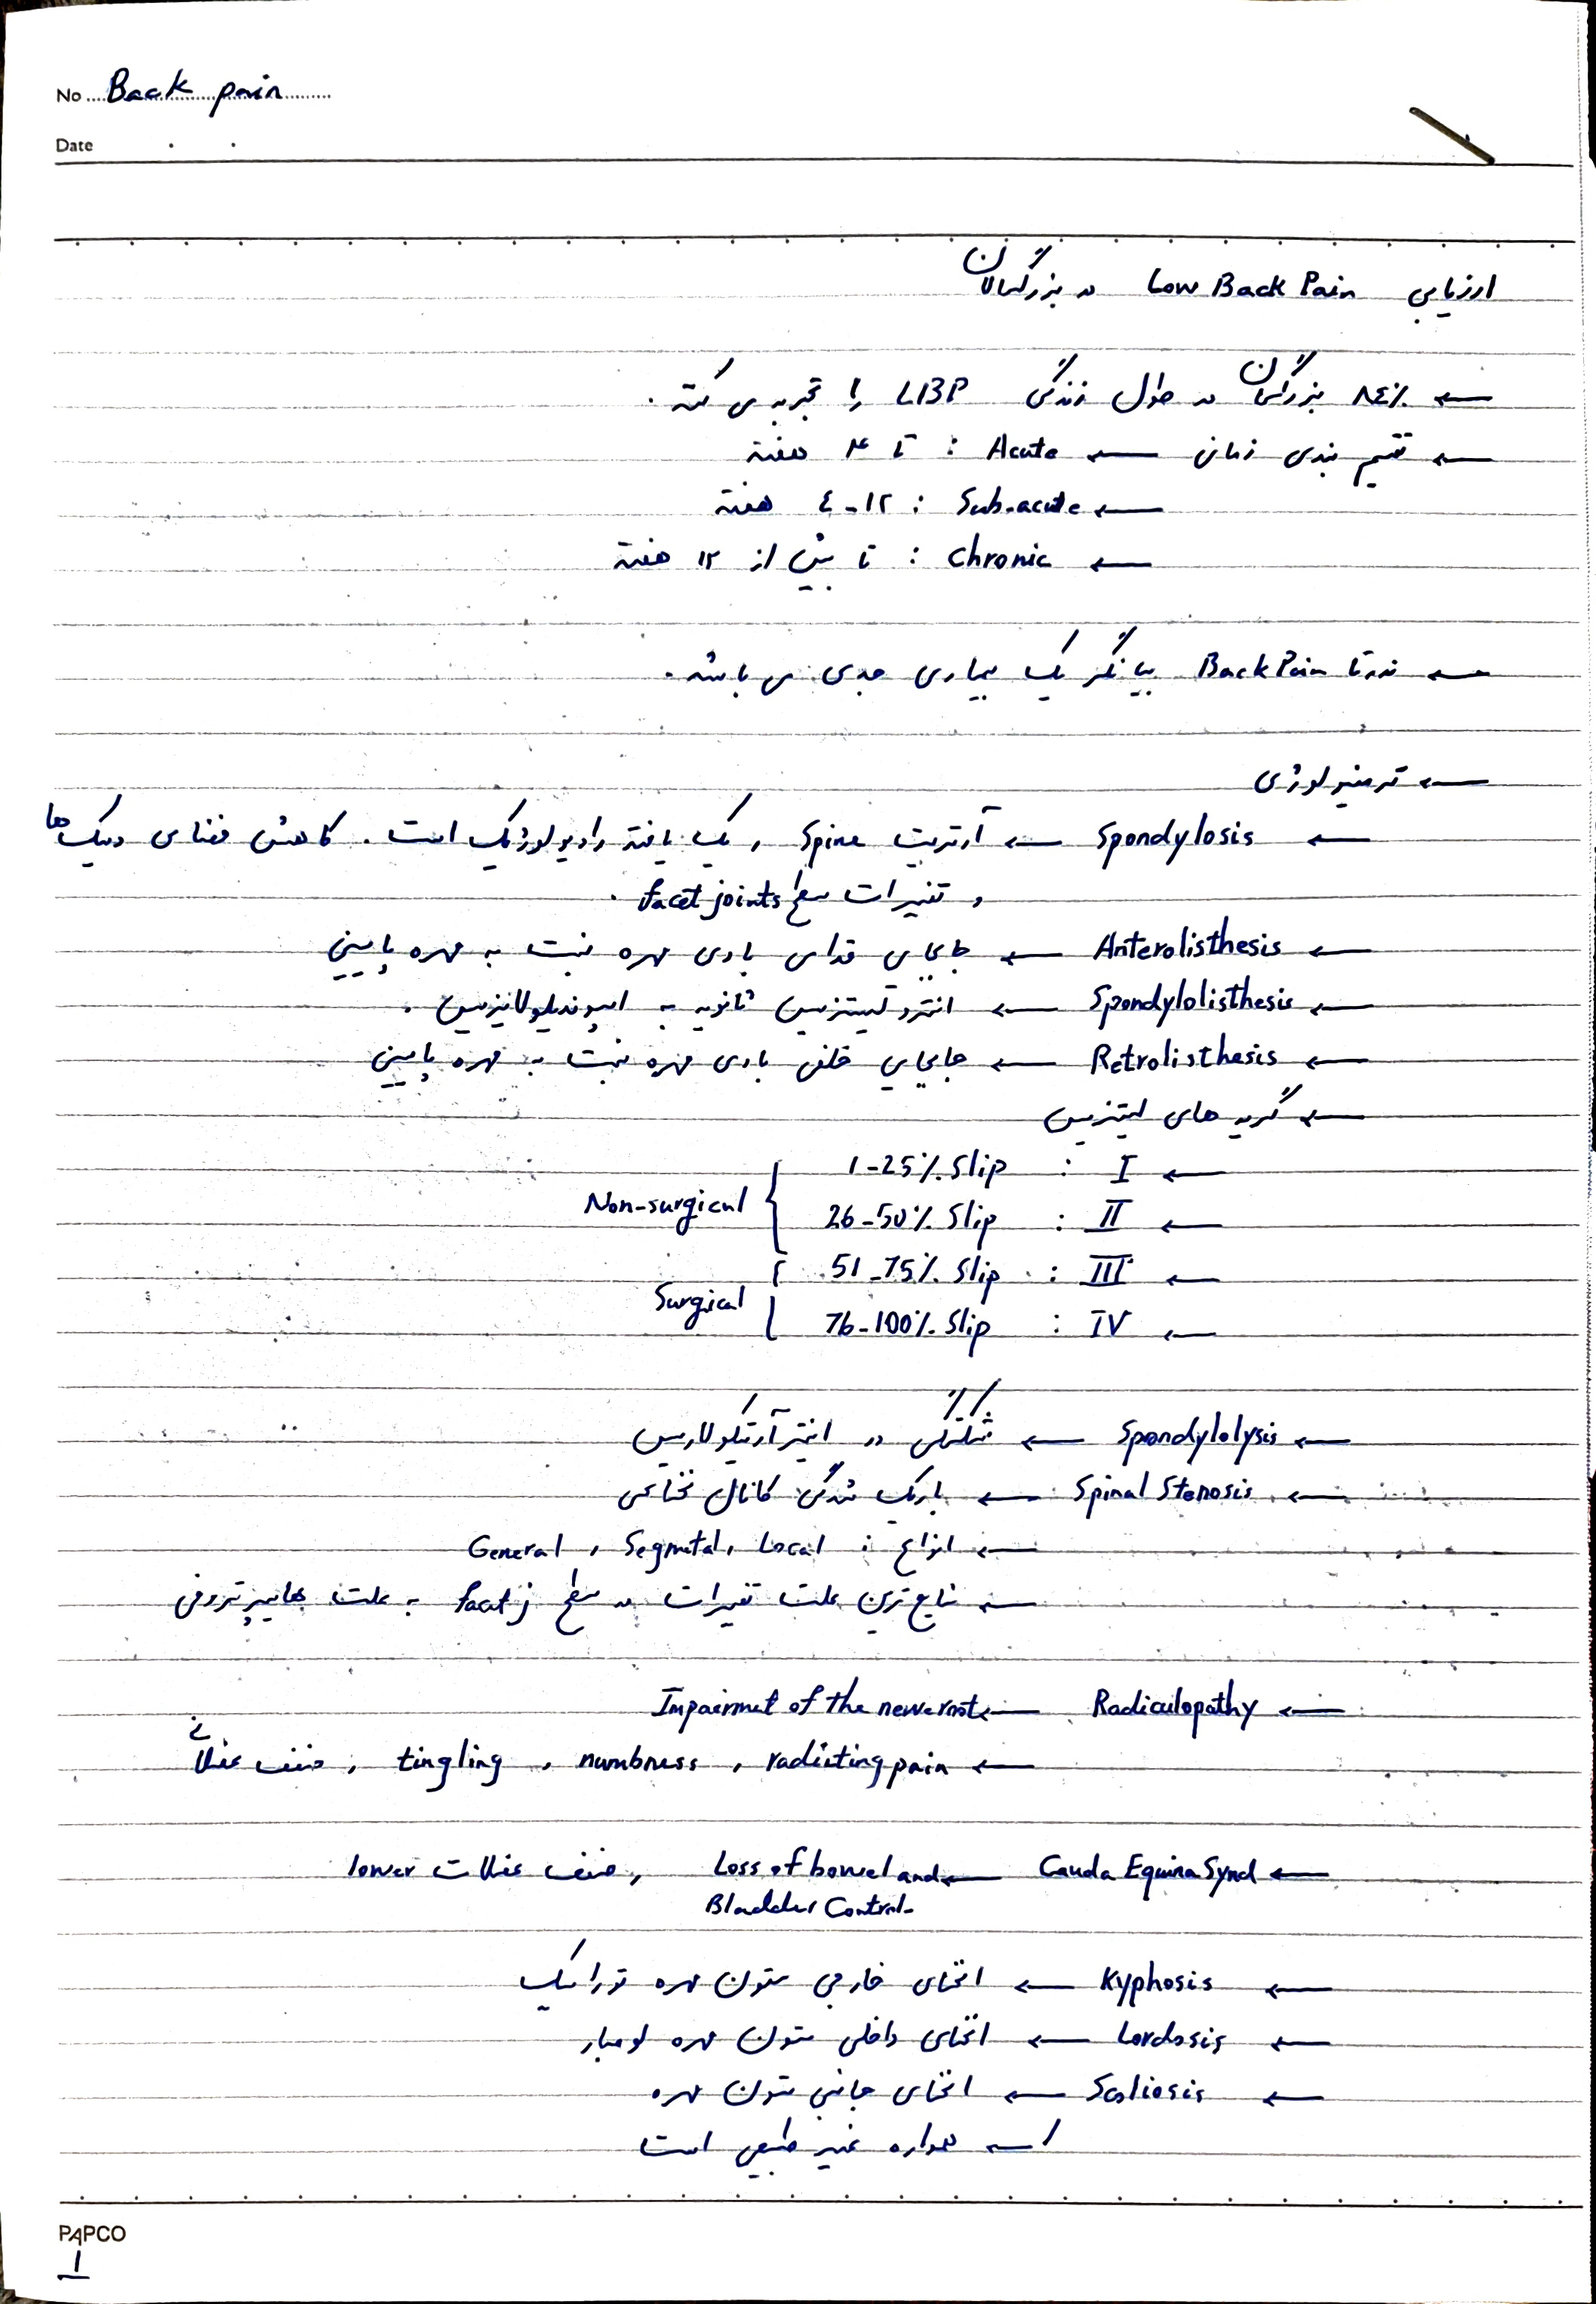
\includegraphics[width=\textwidth,height=0.88\textheight,keepaspectratio]{images/pic01.jpg}
\end{center}
\clearpage
\begin{center}
\textbf{تصویر 2}\par
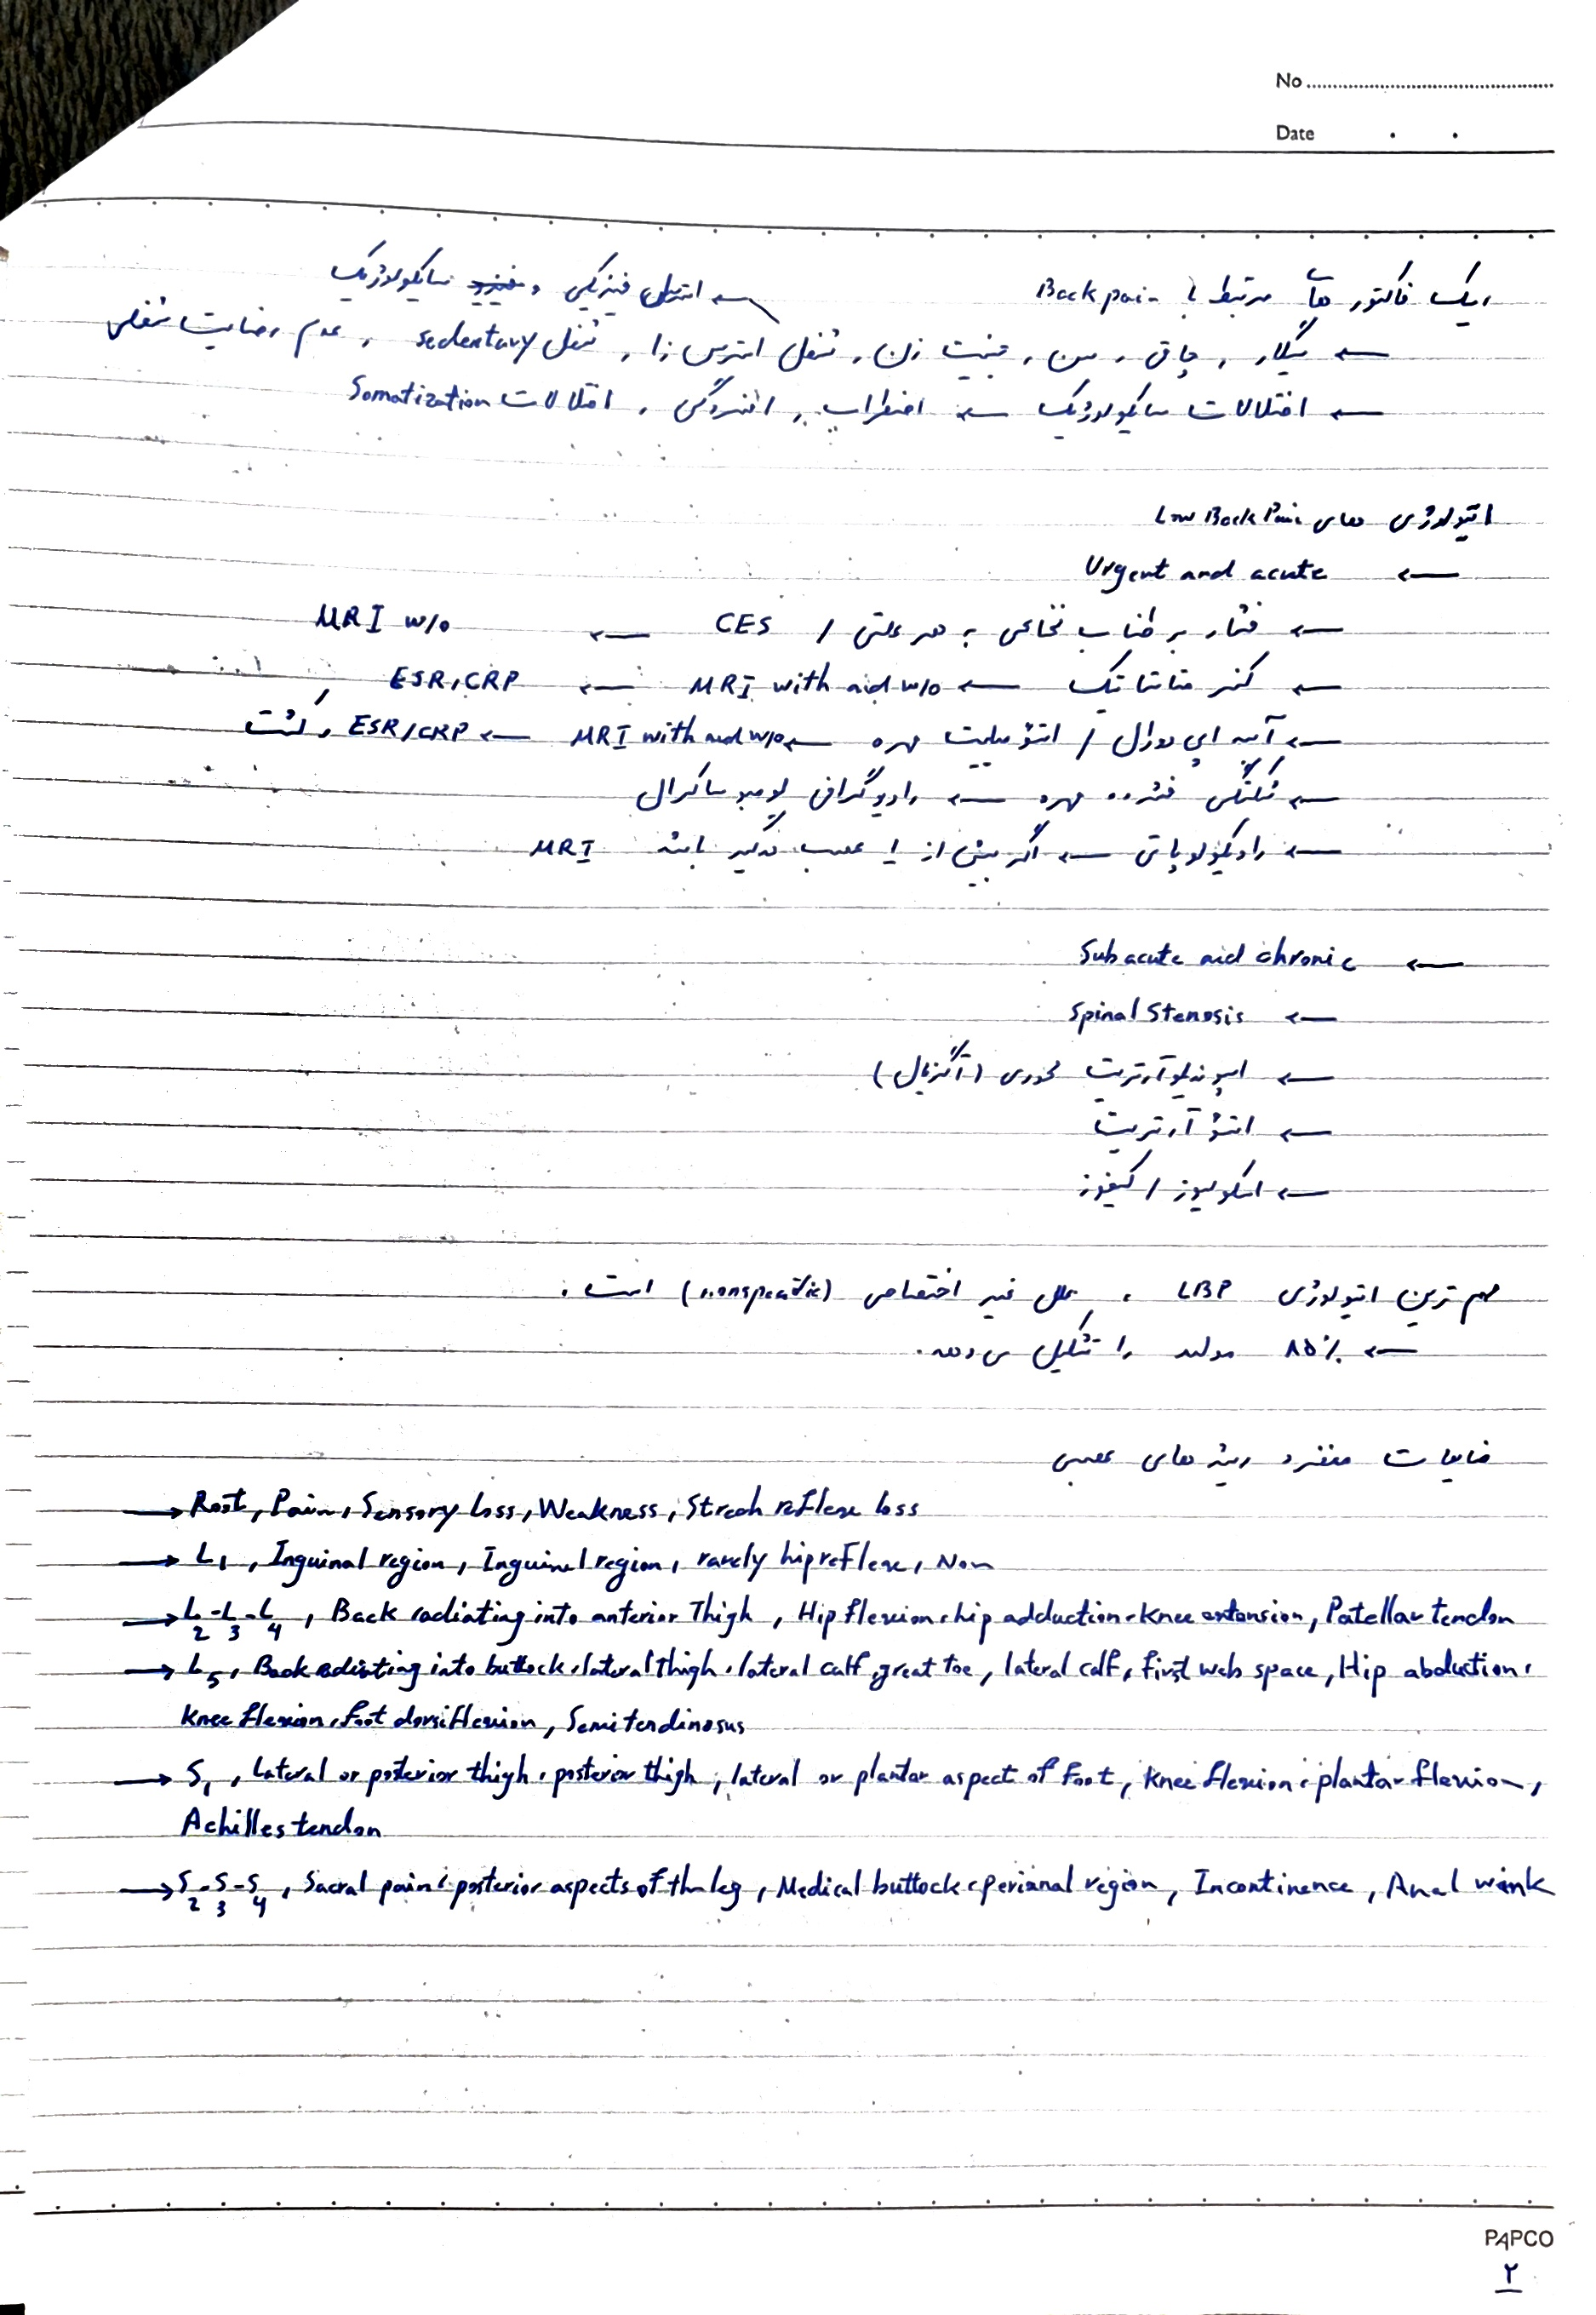
\includegraphics[width=\textwidth,height=0.88\textheight,keepaspectratio]{images/pic02.jpg}
\end{center}
\clearpage
\begin{center}
\textbf{تصویر 3}\par
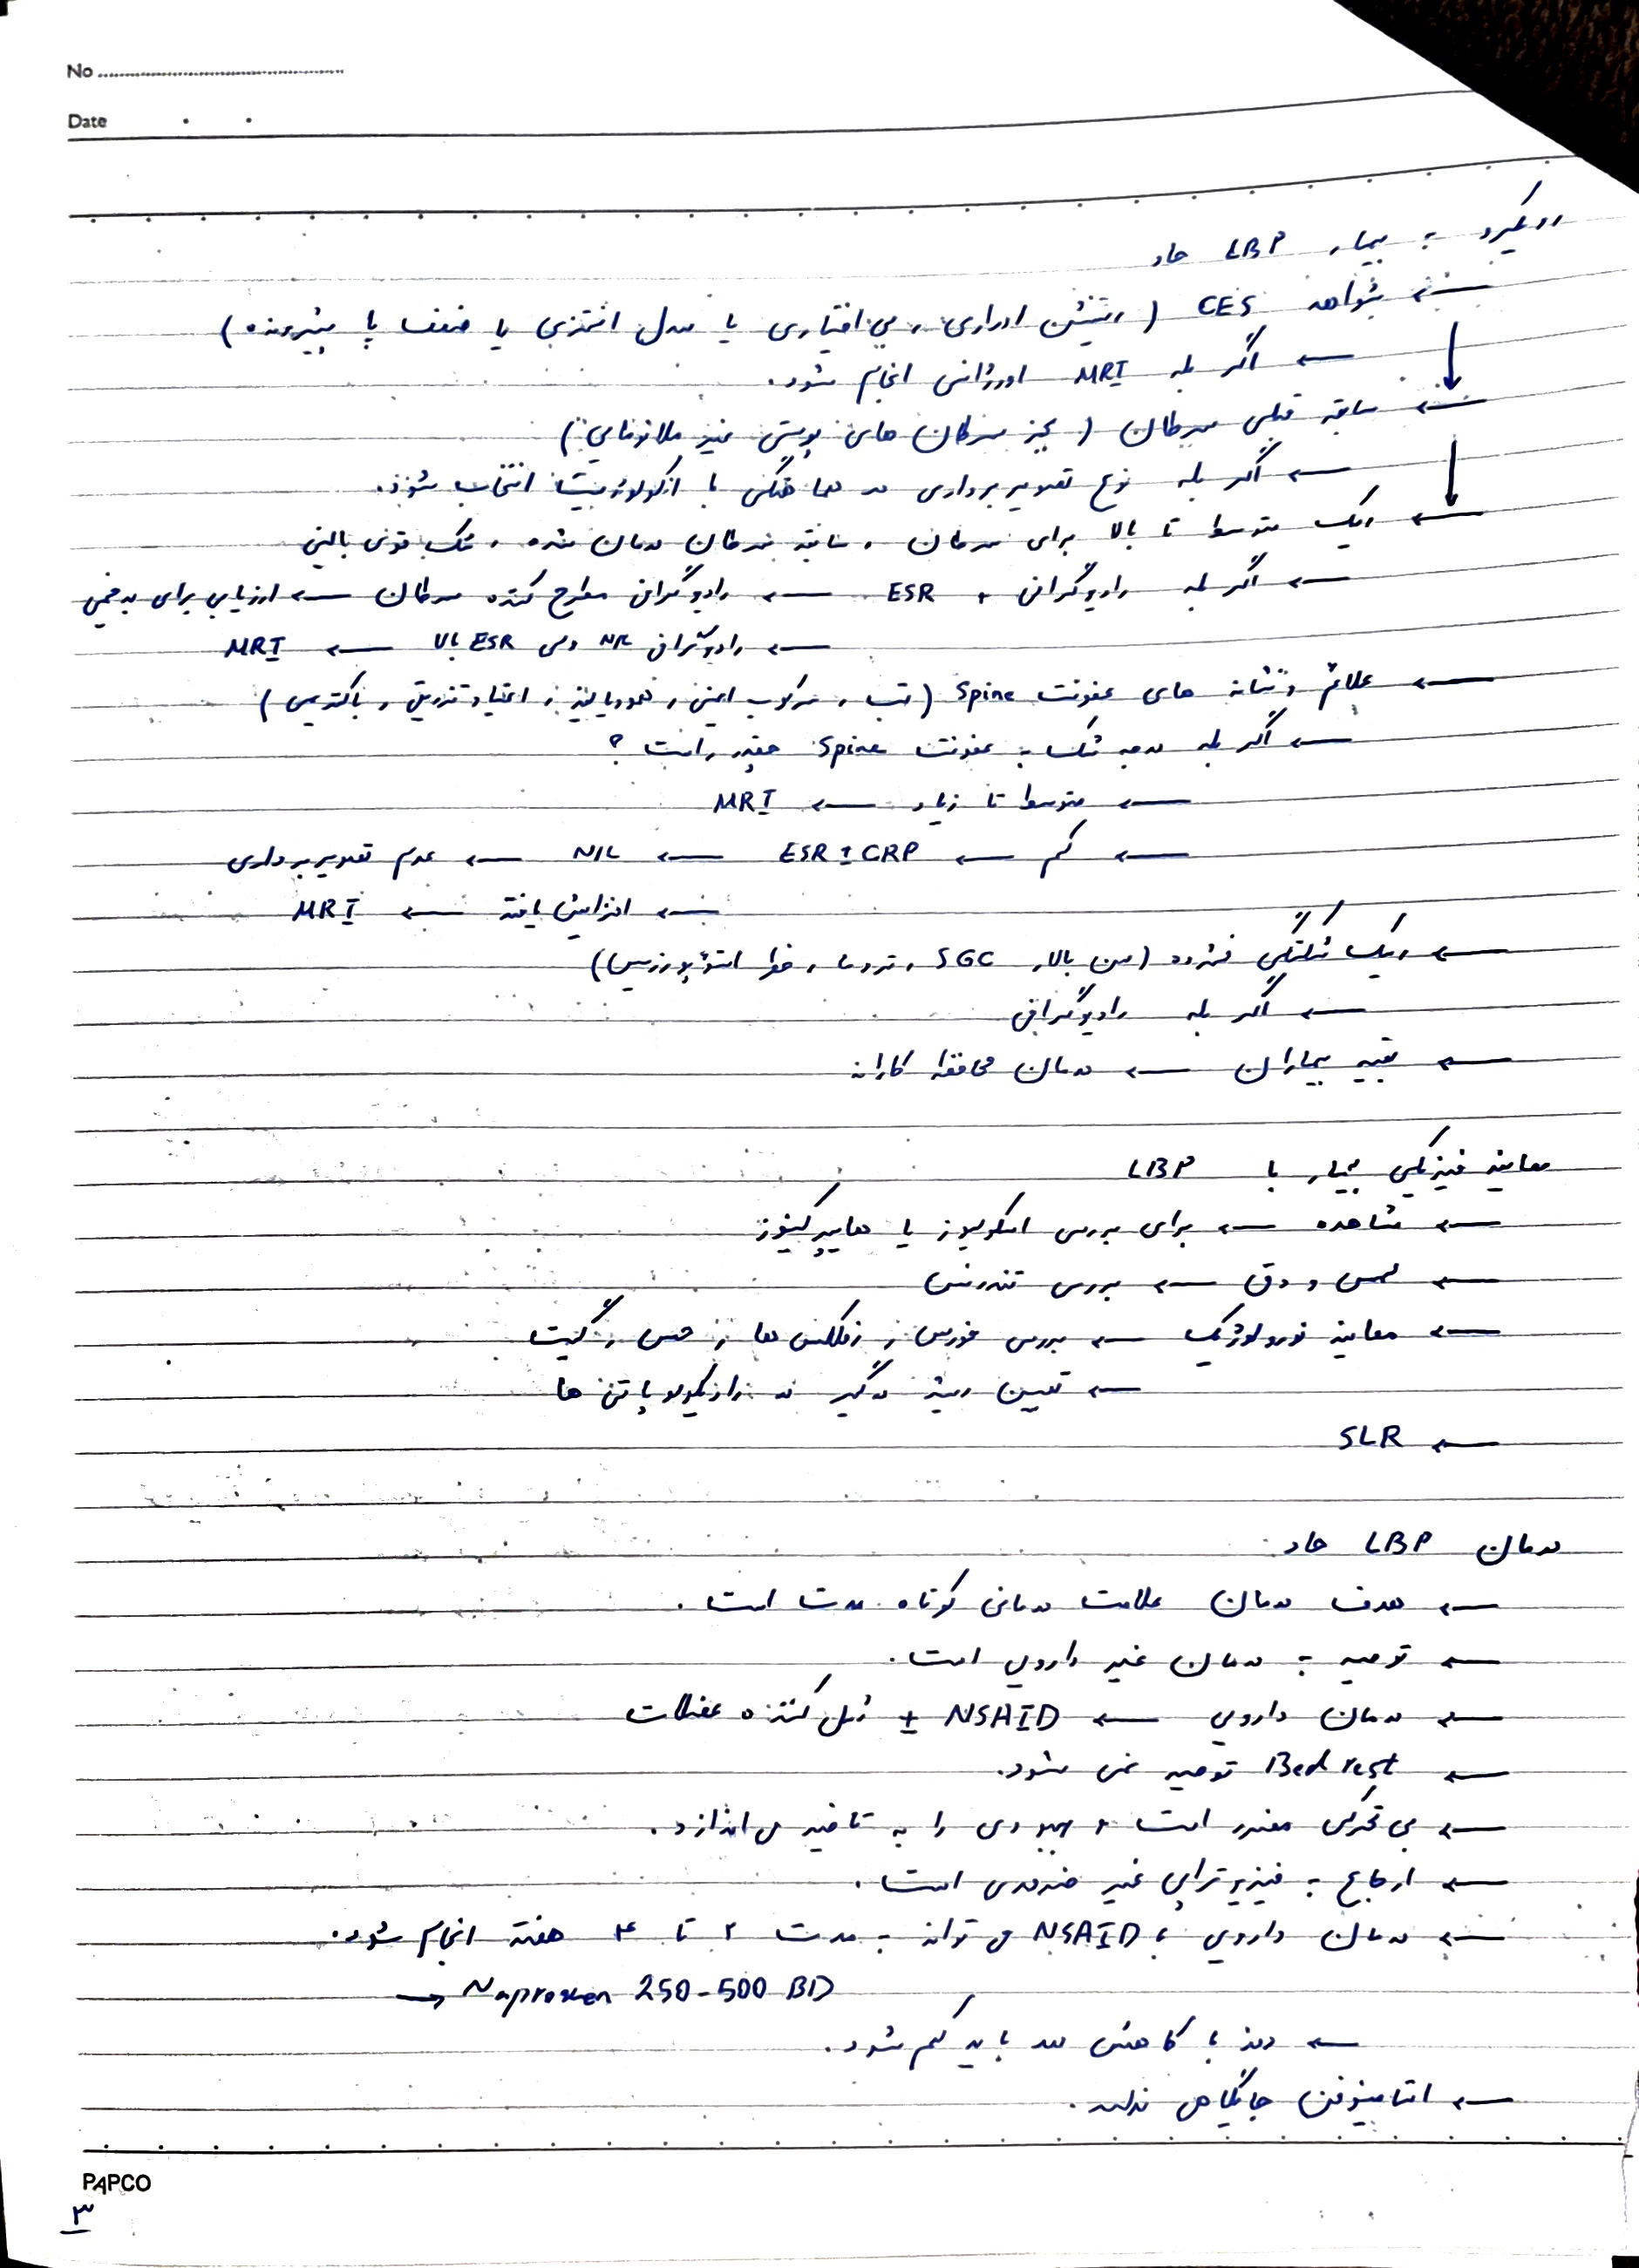
\includegraphics[width=\textwidth,height=0.88\textheight,keepaspectratio]{images/pic03.jpg}
\end{center}
\clearpage
\begin{center}
\textbf{تصویر 4}\par
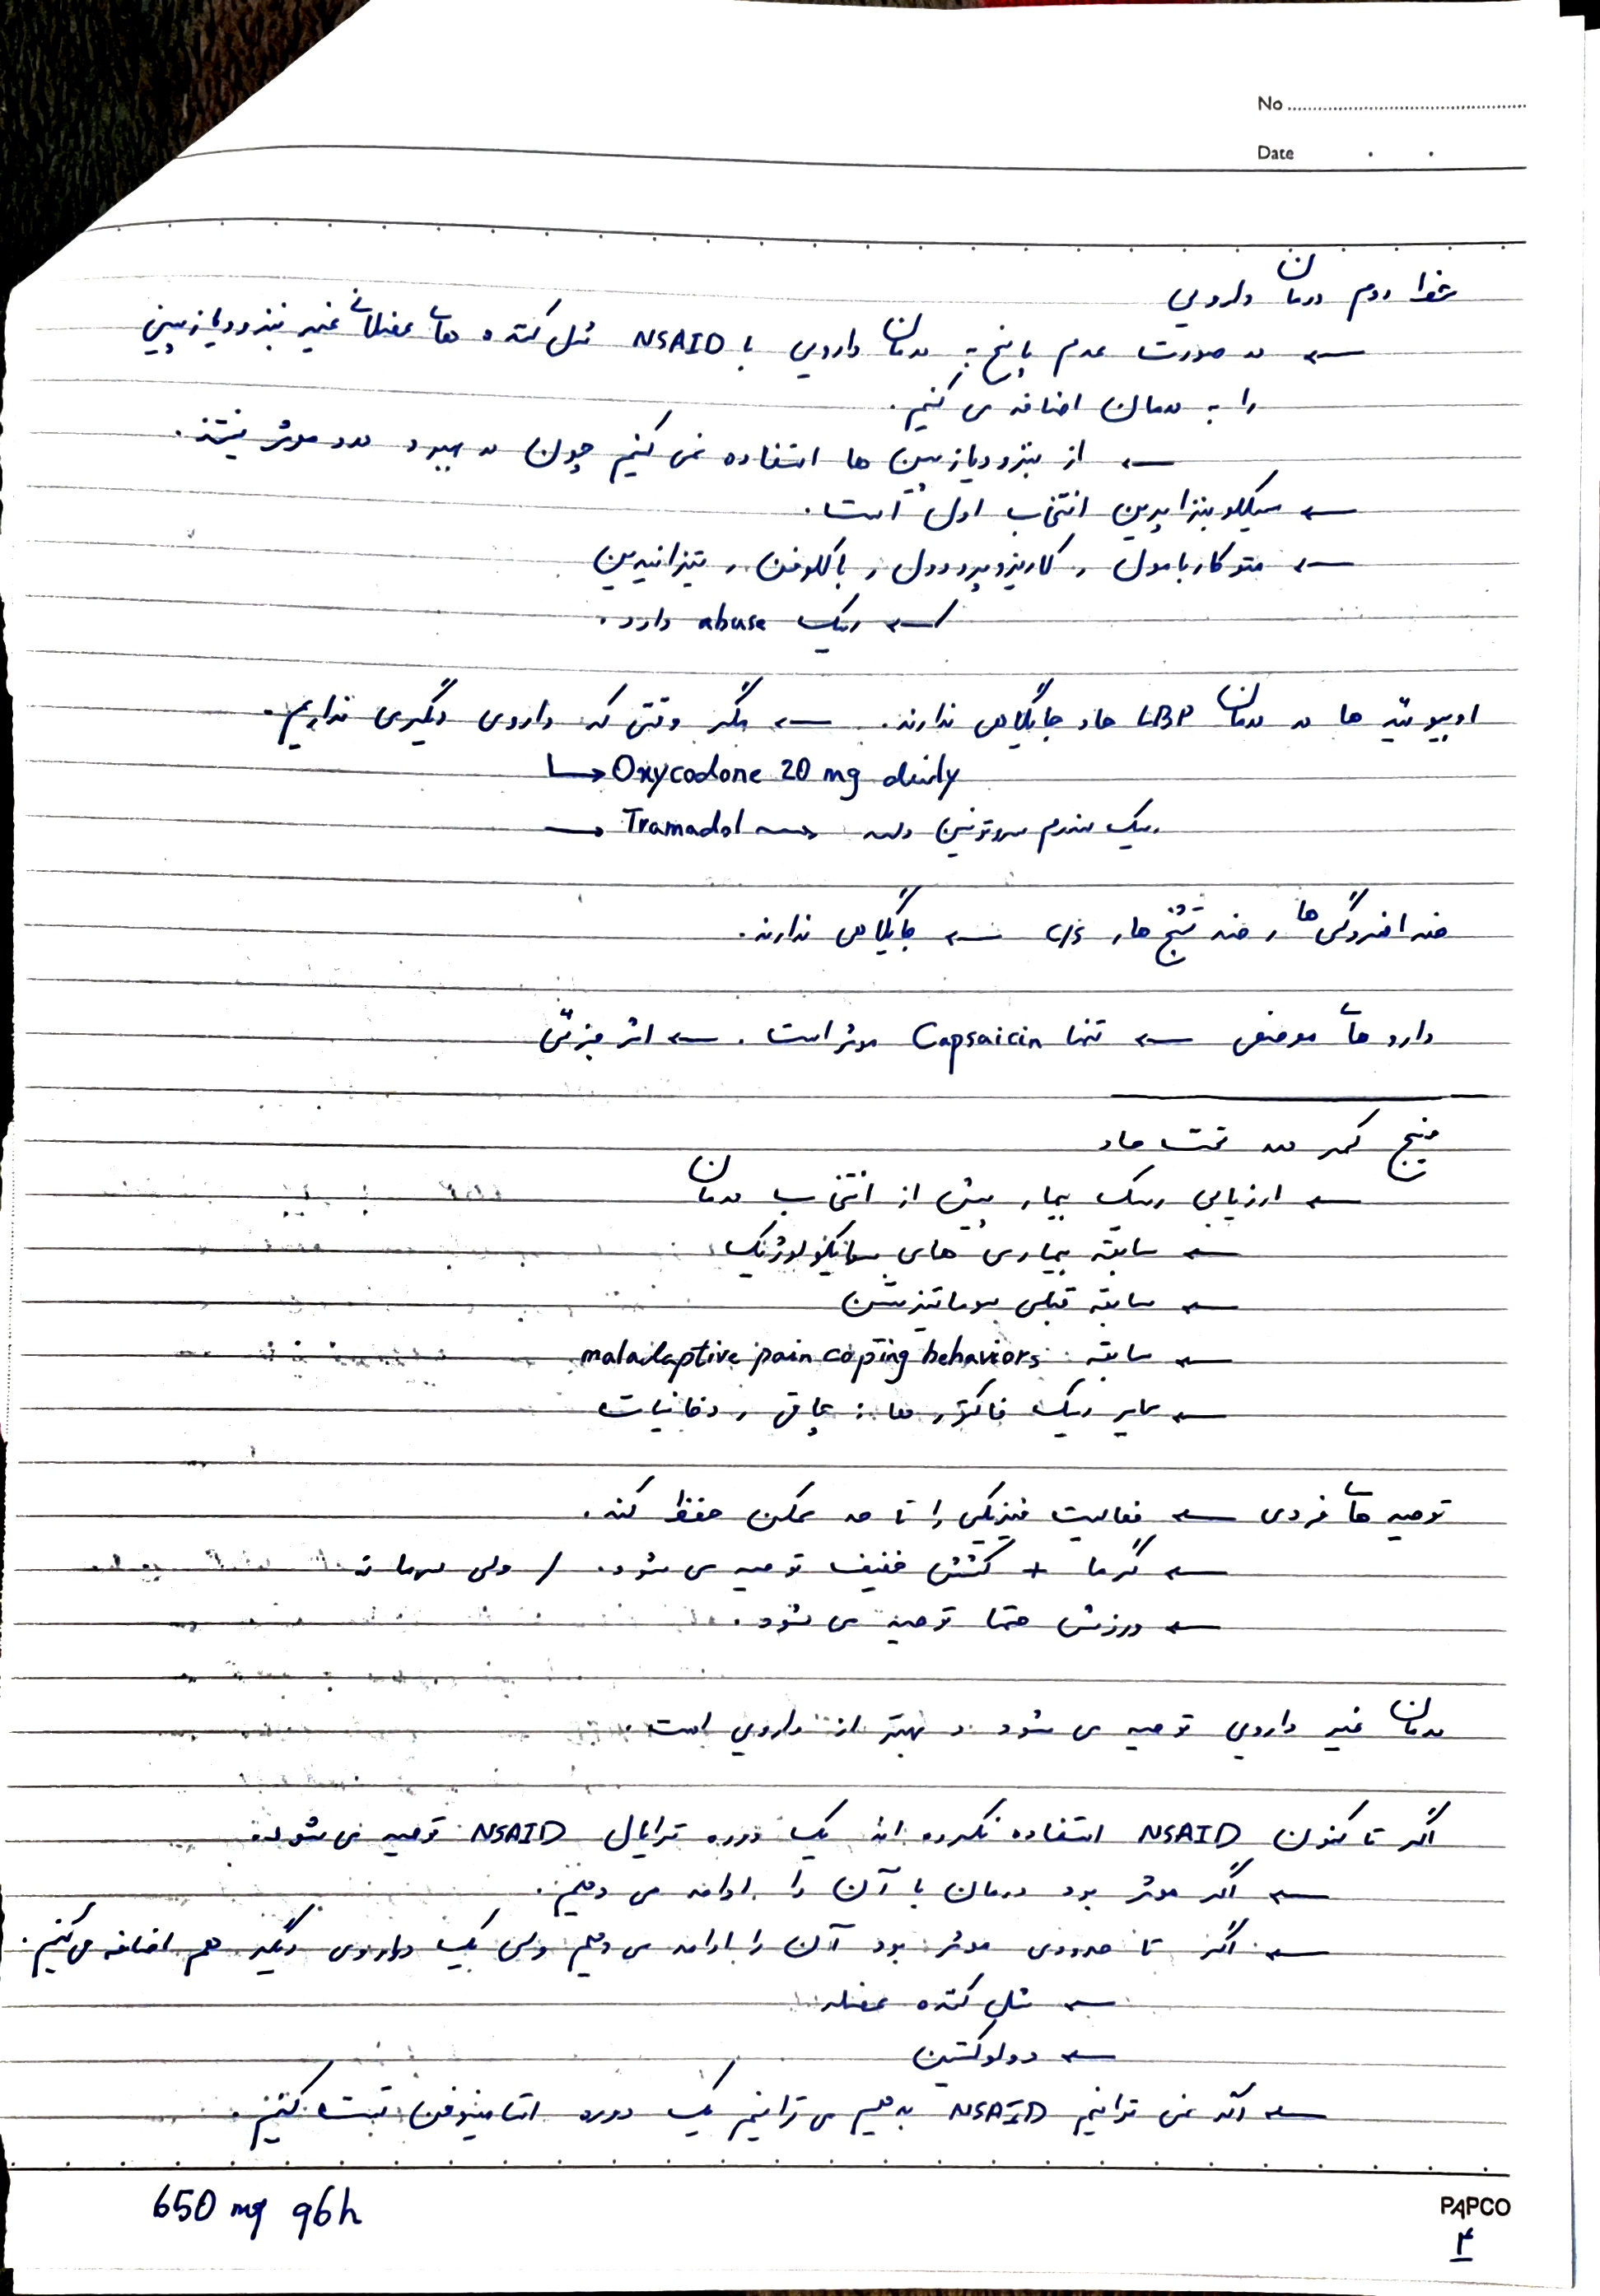
\includegraphics[width=\textwidth,height=0.88\textheight,keepaspectratio]{images/pic04.jpg}
\end{center}
\clearpage
\begin{center}
\textbf{تصویر 5}\par
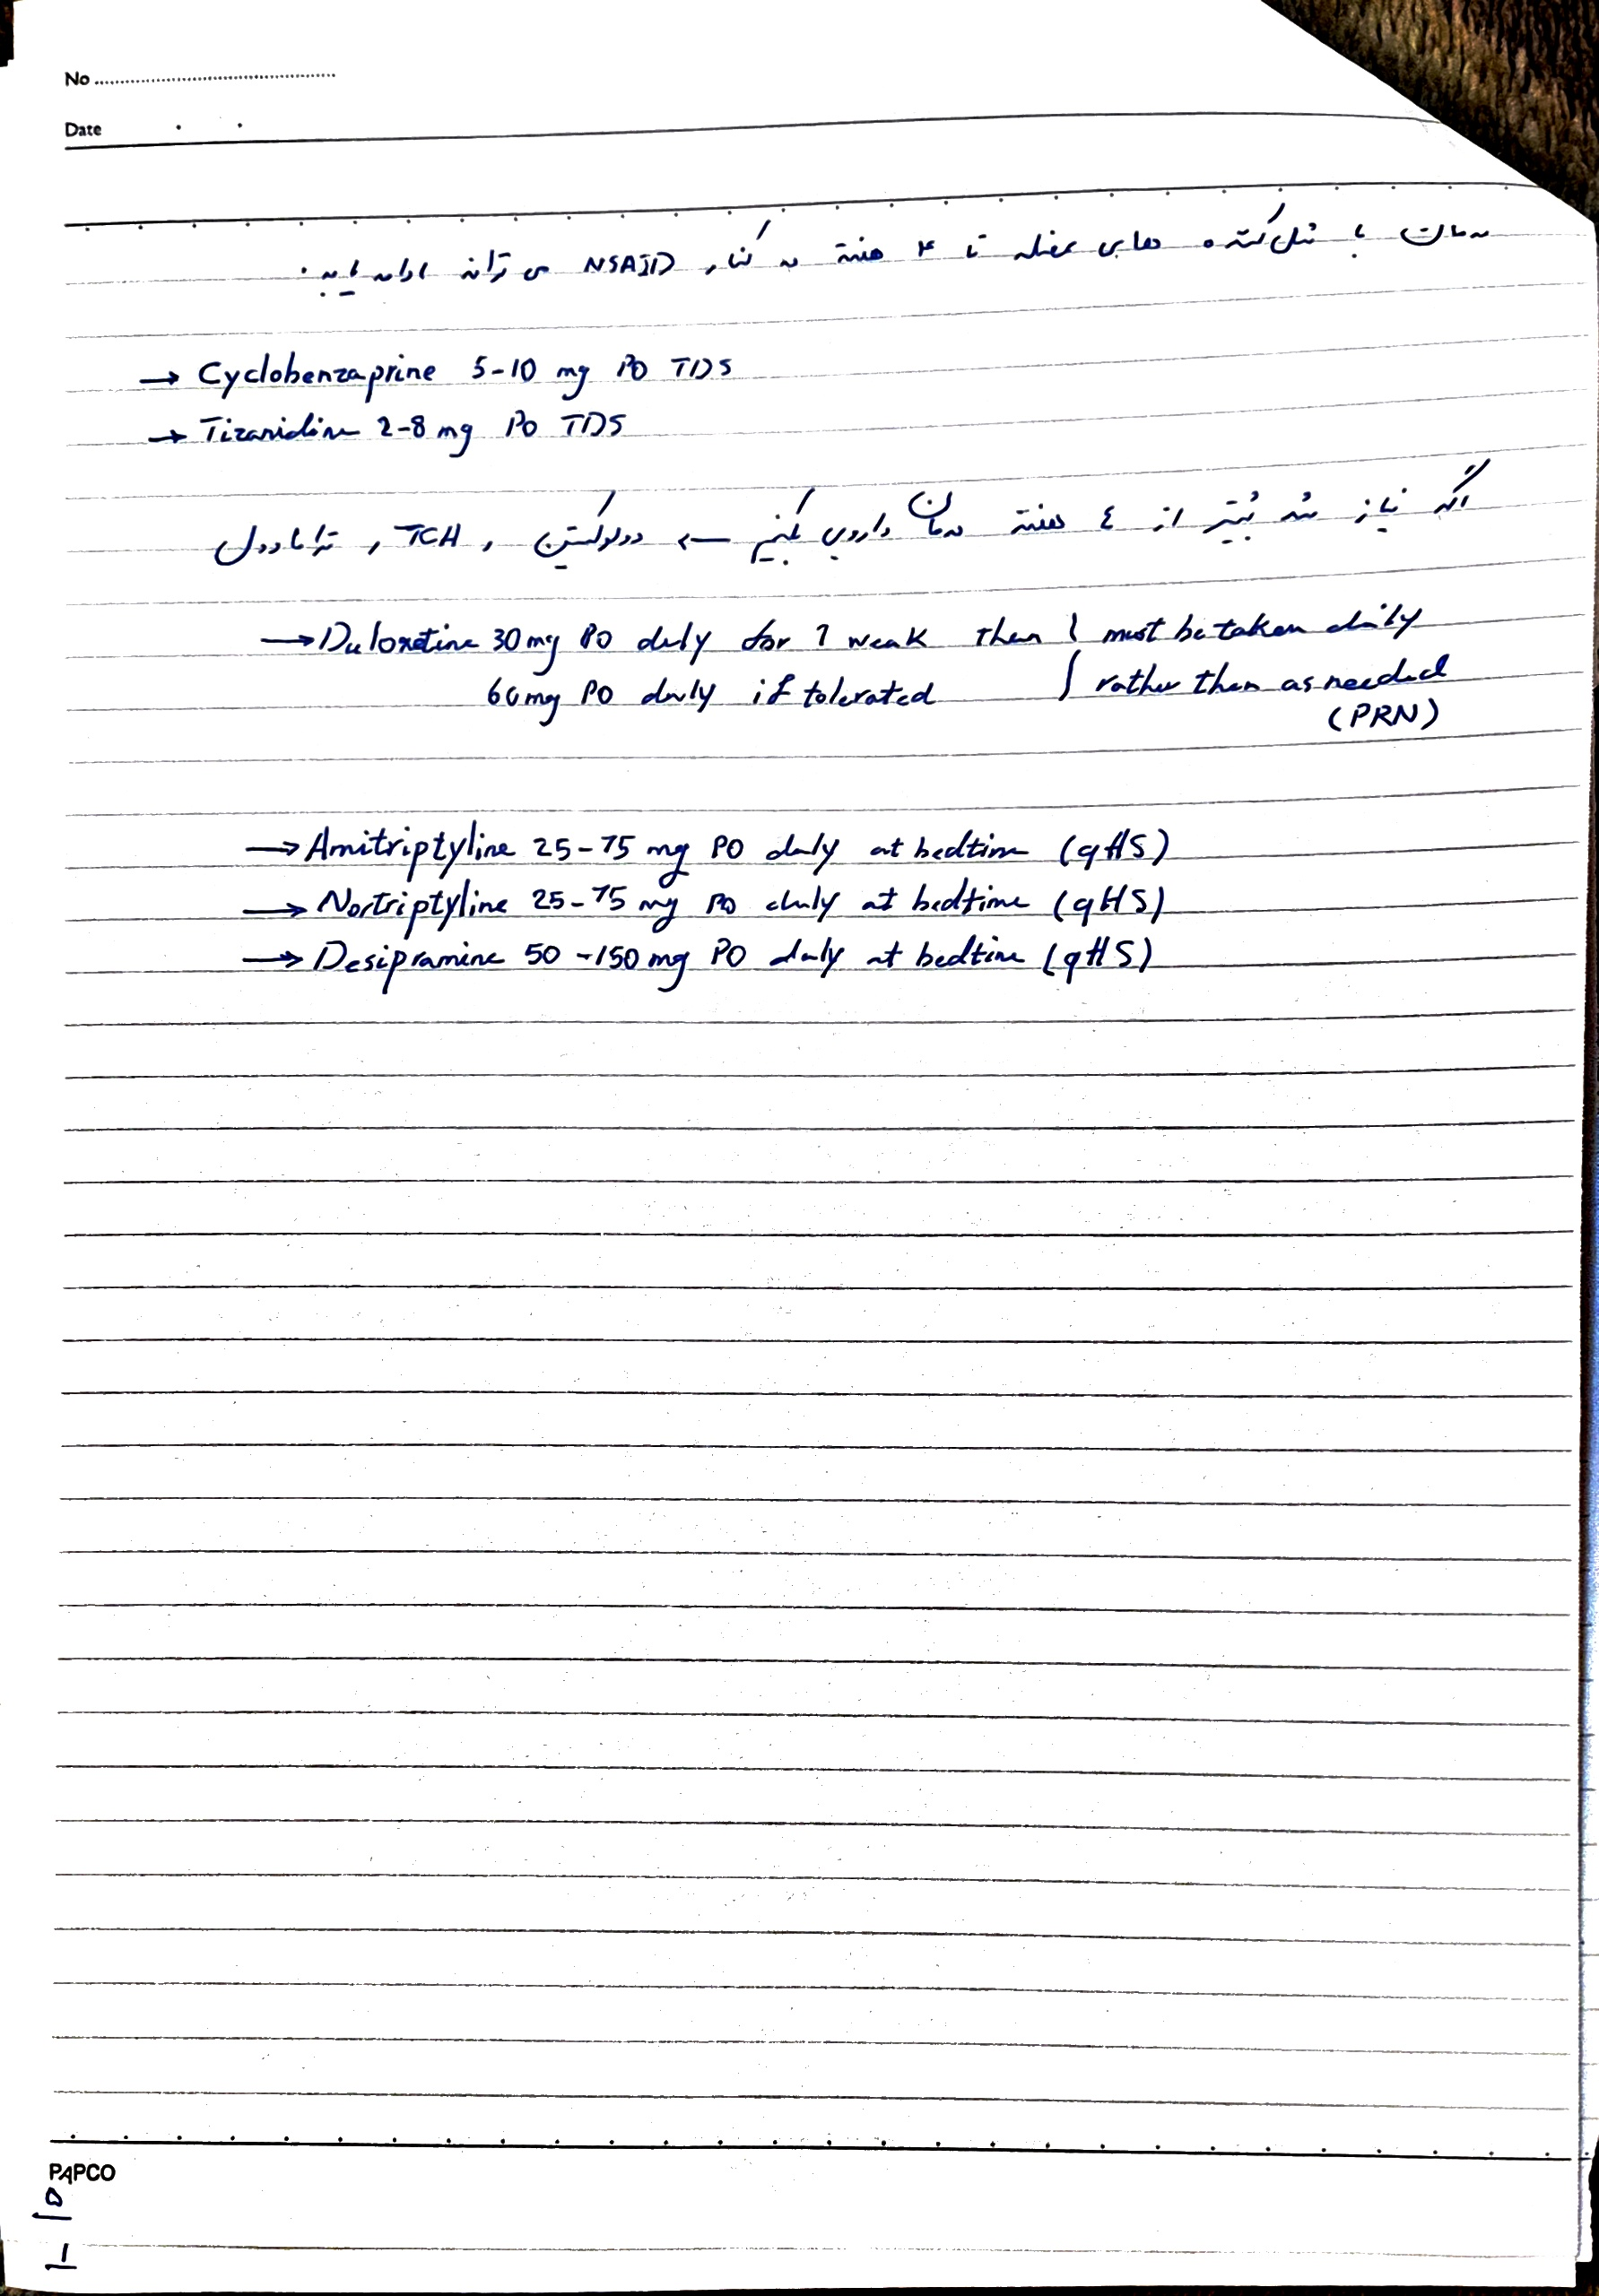
\includegraphics[width=\textwidth,height=0.88\textheight,keepaspectratio]{images/pic05.jpg}
\end{center}
\LBPfinish
